\documentclass[13pt	]{beamer}
\usepackage{lipsum}
\usepackage{tikz}
\usepackage{verbatim}
\usepackage{graphicx}
\addtobeamertemplate{navigation symbols}{}{%
    \usebeamerfont{footline}%
    \usebeamercolor[fg]{footline}%
    \hspace{1em}%
    \insertframenumber
}
\setbeamercolor{footline}{fg=black}
\setbeamerfont{footline}{series=\bfseries}
 
\usetikzlibrary{calc,trees,positioning,arrows,chains,shapes.geometric,
decorations.pathreplacing,decorations.pathmorphing,shapes,matrix,shapes}
\tikzstyle{decision} = [diamond, draw, fill=blue!20, text width=4.5em, text badly centered, node distance=3cm, inner sep=0pt]
\tikzstyle{block} = [rectangle, draw, fill=blue!20, text width=15em, text centered, rounded corners, minimum height=3em]
\tikzstyle{line} = [draw, -latex']
\tikzstyle{cloud} = [draw, ellipse,fill=red!20, node distance=3cm,minimum height=2em]
\newcommand\Fontvi{\fontsize{6}{7.2}\selectfont}
%\usepackage{beamerthemeBoadilla}
%\usepackage{media9}
\usepackage[labelformat=empty,font=small,format=hang,labelfont=bf,up,textfont=it,up]{caption} 
\title{\large\textsc{Trajectory Tracking Of a Small Size Quadrator Using NMPC}}
\date{Nov 13, 2014}
%\author{} 
%\beamersetuncovermixins{\opaqueness<1>{25}}%{\opaqueness<2->{15}}

\begin{document}

\begin{frame}
\titlepage
\begin{center}

\textsf{\footnotesize Bahadir Kocer, Fabian Girribach , Ramin Zohouri}\\
%\textsf{\footnotesize Maren Bennewitz, Martin Riedmiller}\\
%\textsf{\footnotesize Humanoid Robots Lab}\\
\textsf{\footnotesize NOCEO Summer School 2015}\\
\text{\footnotesize University of Freiburg}
%\begin{figure}

%\includegraphics[scale=0.10]{img/Kinect.jpg}
%\end{figure}
\end{center}
\end{frame} 


\begin{frame}
\frametitle{Motivation}
\begin{itemize}
\item Control challanges of Quadrotor:
\subitem Under actuated dynamics
\subitem Strongly coupled non-linearities
\subitem Uncertain paraeters
\subitem Open loop unstable
\begin{figure}
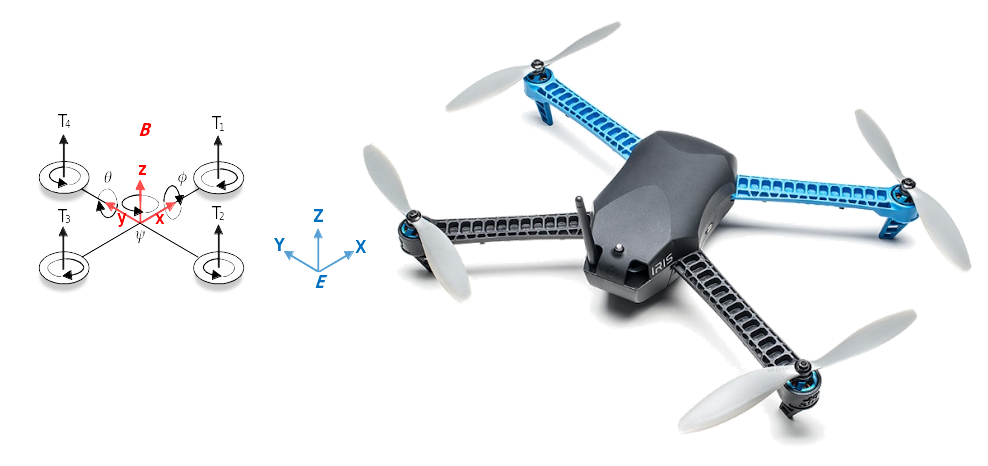
\includegraphics[scale=0.3]{./figures/quad.png}
\caption{\tiny Quadrator by 3D-Robotics.}
\end{figure}
\end{itemize}


\end{frame}

\begin{frame}
\frametitle{Dynamic Model Of Quadcopter} 
\begin{center}
\fontsize{8}{7.2}\selectfont

%\begin{equation} 
%\begin{split}
\begin{align}
&\ddot{\phi}=\dot{\theta}\dot{\psi}\frac{(I_{yy}-I_{zz})}{I_{xx}} + \dot{\theta}\frac{J_r}{I_{xx}} \Omega_r, \\
&\ddot{\theta}=\dot{\phi}\dot{\psi} \frac{(I_{zz} -\dot{\phi}\frac{J_r}{I_{yy}}, \\
&\ddot{\psi}=\dot{\theta}\dot{\phi}\frac{(I_{xx}-I_{yy})}{I_{zz}}+\frac{l}{I_{zz}} U_4, \\
&\Omega_r +\frac{l}{I_{xx}} U_2;~~\Omega_r +\frac{l}{I_{yy}} U_3, \\
&\ddot{x}=cos(\phi)sin(\theta)cos(\psi)+sin(\phi)sin(\psi) \frac{1}{m} U_1, \\
&\ddot{y}=cos(\phi)sin(\theta)cos(\psi)-sin(\phi)cos(\psi)\frac{1}{m}U_1,\\
&\ddot{z}=g-\big(cos(\phi)cos(\theta)\big)\frac{1}{m} U_1. \\

\end{align} 
%\end{split}
%\end{equation}
\end{center}
\end{frame}

\begin{frame}
{Problem Formulation}
\begin{align}
\text{minimize}&&\int_{0}^{T} || \left[
\begin{array}{c}
x(t)\\
u(t)\\
\end{array}
\right]-y(t) ||_{W} ^{2} dt + || x(T) - y(T) ||_{W_N}^ {2} //
\text{subject to} x(0) = && \hat{x}_0,
                        && \dot{x} = f(x(t), u(t)),
                        && 0 \leq u(1) \leq 10,
                        && -7.5 \leq u(2) \leq 0.5,
                        && -7.5 \leq u(3) \leq 7.5,
                        && -7.5 \leq u(4) \leq 7.5,
                       -7.5  \ u \leq  7.5,
                        && -7.5 \leq v \leq 7.5,
                        && -7.5 \leq w \leq 7.5,
\end{align} 
\end{frame}

\begin{frame}
\frametitle{Results}
\begin{table}[h!] 
  \caption{Tricopter Parameters} 
\begin{center} 
\begin{tabular}{|c|c|c|} 
  \hline 
  Paremeter & Value (Unit) \\ 
  \hline
  $Controller$ & $NMPC$ \\ 
   \hline
  $Hessian Approximation$ & $Gauss Newton$ \\ 
   \hline
  $Discretization Type$ & $Multiple Shooting$ \\ 
   \hline
  $Sparse QP Solution$ & $Full Condensing$ \\ 
   \hline
  $Integrator Type$ & $Implicit Runge Kutta$ \\ 
   \hline 
  $QP Solver$ & $QP_QPOASES$ \\ 
   \hline 
  $Tracking Error (RMSE)$ & $0.5007$ \\ 
    \hline 
  $Controller Effort$ & $204.769$ \\ 
    \hline 
  $CPU Time$  & $5.058$  \\ 
    \hline 
  $Iteration Number$ & $1$ \\ 
    \hline 
  $Prediction Horizon$ & $40$  \\ 
    \hline 
\end{tabular} 
\end{center} 
\end{table}
\end{frame}




\begin{frame}
\begin{center}
Question ?
\end{center}
\end{frame}


\end{document}
